\documentclass[conf]{new-aiaa}
%\documentclass[journal]{new-aiaa} for journal papers
\usepackage[utf8]{inputenc}

\usepackage{graphicx}
\usepackage{subcaption}
% \usepackage[demo]{graphicx}
\usepackage{tikz,pgfplots}
\usepackage{amsmath, bm, amssymb,amsfonts,amsthm}
\usepackage{float}
\usepackage[version=4]{mhchem}
\usepackage{siunitx}
\usepackage{longtable,tabularx}
\usepackage{makecell}
\usepackage[labelfont=bf]{caption}
 \usepackage{setspace}
\usepackage[table]{xcolor}
\usepackage[x11names,dvipsnames,table]{xcolor} %for use in color links
\usepackage{colortbl}

\setlength\LTleft{0pt} 

\title{Topographical Mapping via a Micro-Quadcopter}

\author{ Parthiv V. Kukadia, Salam Mulhem, Ani Pirosmanishvili, and Pallavi Ravada \footnote{Student, Department of Aerospace Engineering, 302 Transportation Building, 104 S Mathews Ave, Urbana, IL 61801, USA.}}
\affil{University of Illinois at Urbana-Champaign, Champaign-Urbana, Illinois, 61801}
\date{May 2021}

\begin{document}

\maketitle
\begin{abstract}
\label{abstract}
This paper will describe the design, implementation, and verification of a micro-quadcopter for topographical mapping. Topographic mapping has innumerable applications ranging from civilian hiking to military tactical positioning. The focus of this report is leveraging the CrazyFlie’s positioning capabilities for simple topographic mapping of a region of interest. This is motivated by the need to understand poorly mapped environments, such as the surface of different planets. This could enable successful landing of other spacecrafts, as well as facilitate further exploration of those regions. Implementation began with surveying a test area with the drone in a switch back pattern to ensure full coverage of the test section and collection of positional (x,y,z) information. To increase reliability, the drone was flown forward and backwards over the object filled grid, so that the data was collected twice. The geospatial data collected was then visualized in python producing an interactive three dimensional contour plot of the object filled grid. There were some challenges that had to be overcome, one of which was the inability of the custom observer and controller to fulfill flights within the defined RMSE values. Therefore the stock controller and observer of the CrazyFlie drone was used during the tests. The final visualizations were accurate to the real world object filled grid in terms of identifying objects, but not in dimensions. Topographical mapping via a micro-quadcopter provided a detailed visualization of the test grid, and can be applied in mapping larger surfaces using a larger quadcopter.
%Revised topic paragraph 
\end{abstract}

\section{Nomenclature} 
\label{Nomenclature}
{\renewcommand\arraystretch{1.0}
\noindent\begin{longtable*}{@{}l @{\quad=\quad} l@{}}
A & system matrix\\
B & input matrix\\
C & output matrix\\
D & feed-forward matrix\\
y & output vector\\
s & state vector\\ 
i & input vector\\
$o_x$ & x-position of the drone (m)\\
$o_y$ & y-position of the drone (m)\\
$o_z$ & z-position of the drone (m)\\
$\phi$ & roll angle of the drone (rad)\\
$\theta$ & pitch angle of the drone (rad)\\
$\psi$ & yaw angle of the drone (rad)\\
$v_x$ & x direction linear velocity of the drone (m/s)\\
$v_y$ & y direction linear velocity of the drone (m/s)\\
$v_z$ & z direction linear velocity of the drone (m/s)\\
$\omega_x$ & angular velocity about the x-axis of the drone (rad/s)\\
$\omega_y$ &  angular velocity about the y-axis of the drone (rad/s)\\
$\omega_z$ & angular velocity about the z-axis of the drone (rad/s)\\
$\tau_x$ & the drone's torque about its x-axis ($N \cdot m$)\\
$\tau_y$ & the drone's torque about its y-axis ($N \cdot m$)\\
$\tau_z$ & the drone's torque about its z-axis ($N \cdot m$) \\
$f_z$ & net force along the body-fixed z-axis (N)\\
K & non-dimensional angular deflection rate of the trailing edge (controller gains matrix)\\
L & observer gains matrix\\
m & mass (kg)\\
$J_x$ & moment of inertia in the x-direction ($kg m^2$)\\
$J_y$ & moment of inertia in the y-direction ($kg m^2$)\\
$J_z$ & moment of inertia in the z-direction ($kg m^2$)\\
g & gravity ($m/s^2)$\\
l & length from edge of the drone to center of the drone (m)\\
$K_F$ & Force coefficient (ND)\\
$K_M$ & Moment Coefficient (ND)\\
\end{longtable*}}

\section{Introduction}
\label{introduction}
% This section must prepare the reader to understand the rest of your report. (What will you do? Why is it important? Who else has done similar things? How will your report be organized? To what, in particular, should readers pay attention?) This section must cite at least five references - for example, these can be final project reports that were written by students in prior years (Links to an external site.) (see below).

Topographical mapping provides a detailed record of a land area. The geographic positions and elevations of the region of interest as well as other geographic features can be determined by means of contour lines. A contour line is an imaginary line on the land surface connecting points of equal elevation. The goal of this project is to utilize the CrazyFlie's positioning capabilities to implement topographical mapping. This is motivated by the need to understand unmapped or poorly mapped environments. Topographic mapping by drone also enables easier access to otherwise inaccessible areas due the drone's versatility and ability to take off and fly just about anywhere. In addition, aerial mapping via drone is significantly faster than land based methods due to the labor intensive nature of geospatial data collection [1]. This project bears similarity to one done in Fall 2019 which focused on thermal mapping and another done in Fall 2014 which investigated sonar mapping [2,3]. Both projects produced contour maps of regions of interest. The former visualized the temperature gradient across and room while the latter plotted the intensity of audio signals over the test area. The current work also seeks to create a contour map over an area of interest, however the data being visualized will be topographic. 

The drone documents elevation data with a downward facing sensor underneath the CrazyFlie. This allows the drone to maintain a very precise z-position altitude by using the distance to the floor as absolute height [4]. This project takes advantage of the variable definition of "floor" to obtain altitude information about objects in the region of interest. The CrazyFlie maintains an absolute height above the floor directly below it. If the height of the floor were to suddenly change, i.e. placing a hand underneath the z-range sensor, the drone would readjust itself to maintain the same height above the hand or general obstacle. Through comparing the relative and absolute position of the drone the elevation of the object can be extracted. There are a multitude of use cases for topographic mapping ranging from recreational activities such as hiking to more technical disciplines such as designing any infrastructure project or flood prediction. 

In order to fully map out an area the drone will follow a lawnmower pattern over a region of specified size, collecting z-position data. This is similar to a project done in Fall 2014 which investigated coverage algorithms for a rectangular region of area [5]. The coverage method employed in this project will be the switchback method as termed in the 2014 project. This method was chosen due to its simplicity to implement, as opposed to the other method discussed in the 2014 project: random coverage mapping. There are marked advantages to the random coverage method, however the added implementation complexity as well the nature of topographical mapping dictate the switchback method to be the optimal choice. This flight path was also chosen in another project from Fall 2014 focused on wildlife surveillance to ensure full coverage of the area being surveyed [6]. It should be noted that the previous work maintained the drone at constant altitude throughout the aerial survey while the current investigation makes use of varying altitude. 

This report will provide the methodology for implementing topographic mapping utilizing the drone foundation developed in the labs. The report will first go through the controller and observer design and implementation followed by the methods employed to enable topographic mapping. Then the results of the flight tests will be visualized and discussed. Finally the big takeaways of the project will be presented as well as potential future work in topographical mapping.




\section{Mission Design}

With the goal of topographical mapping in mind, refinement of scope and the establishment of a plan was required. 

\subsection{Scope}
In the real world, topographical drone applications would require the ability to traverse large areas across many environments while encountering obstacles of unknown and drastically varying size. The team recognized immediately that the scope of the project needed to be refined first to ensure that a feasible goal was established. 

\subsubsection{Grid and Flight Pattern}
First, it was decided that a fixed test space was needed such that it balanced room for adequate data collection and the ability to rapidly iterate. Too large of an area would take too long to fly over and would require more free space, while too small of an area wouldn't provide enough flight time and could potentially lead to minimal space to perform maneuvers. A 1.5 meter square grid was selected as the test space.

A space-driven flight pattern was then created and standardized to be used across all tests performed. This was another instance of refining scope - though in the real world drones may fly in unique patterns with complex maneuvers, this predetermined flight path allows for simplicity and repeat-ability. The drone was flown at a constant height of 0.45 meters, taking off from the origin and completing a forward lawnmower pattern of fixed width across the grid. Once complete, the drone would engage in a reverse lawnmower pattern, flying again in fixed-width sweeps back to the origin where it would land. The grid and flight path are shown below in Figure \ref{fig:lawnmower}. The
drone begins at the bottom left corner which was be defined as the origin (0,0). The end of the grid in coordinate system
is (1.5,1.5). The dark blue lines depict the path of the drone moving forward to the end of the grid. The red dashed line depicts the drone returning back to origin from the end.

\begin{figure}[H]
  \centering
  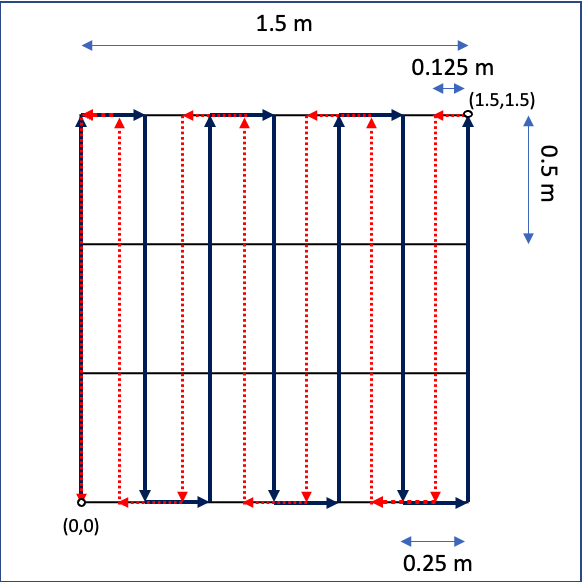
\includegraphics[width=0.6\linewidth, height=0.6\linewidth]{Technical/FP.png}  
  \caption{Drone forward (navy) and backward (red) lawnmower flight pattern on square grid}
  \label{fig:lawnmower}
\end{figure}

\subsubsection{Obstacles and Object Detection}
By the nature of their application, drones used for topographical mapping are collecting data on objects of unknown dimensions. Inherently, drones that are flying close to the objects of interest must be equipped with obstacle avoidance capabilities such that they do not collide with the things they are studying. To minimize this added level of complexity, the project scope was refined to only detect objects' dimensions, rather than also actively try to avoid them. To do this, objects of known dimensions were used in this study which allowed the aforementioned constant flight height to be set at a value higher than the tallest obstacle. This ensured that the drone was always flying high enough to never crash into an object. In addition to simplifying obstacle avoidance, having objects of known dimensions gave a baseline to compare drone mapping results against to gauge topographical measurement accuracy.

The number of objects on the grid was set to two, each being detected twice in one flight loop - once during the forward lawnmower sweep and again in the backward sweep. This was done to ensure that the test space wasn't over crowded, and that adequate spacing would allow for clear contrast of measured object heights relative to what was being detected as the floor. It would have been undesirable to produce a plot that was cluttered and hard to read. Additionally, extra spacing ensured that the drone had time to recover between each object detection. Moreover, using two objects of different dimensions allowed a larger, more informative data set to be collected. Object placement on the grid was random, with an example configuration seen in Figure \ref{fig:OFG}.

\begin{figure}[H]
  \centering
  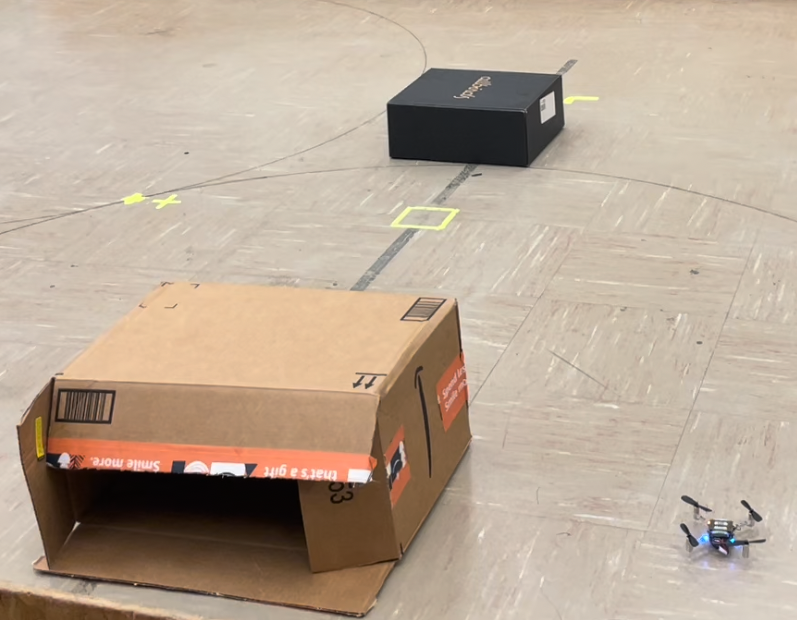
\includegraphics[width=0.5\linewidth]{Technical/OFG.png}  
  \caption{Object Filled Grid}
  \label{fig:OFG}
\end{figure}

\subsection{Milestones}
To ensure that the project was on track to be complete by the end of the semester, a series of milestones were developed to guide the team. Additionally, this helped to set intermediate goals, to allocate time efficiently, and to simplify the process of delegating tasks.

\subsubsection{Milestone 1: Determining Height Collection Method}
This milestone was to understand and implement how to get the absolute and relative z-position of the drone. There were two methods considered: using a loco-positioning system or using the z-position data of the drone. Once the latter method was selected, it was implemented in a flight test where the drone was flown in a straight line over an object of known height. The data was then extracted to see if the
drone was able to provide the x, y, and z position of the object. A visualization of this data is given below in Figure \ref{fig:m1}.

\begin{figure}[H]
  \centering
  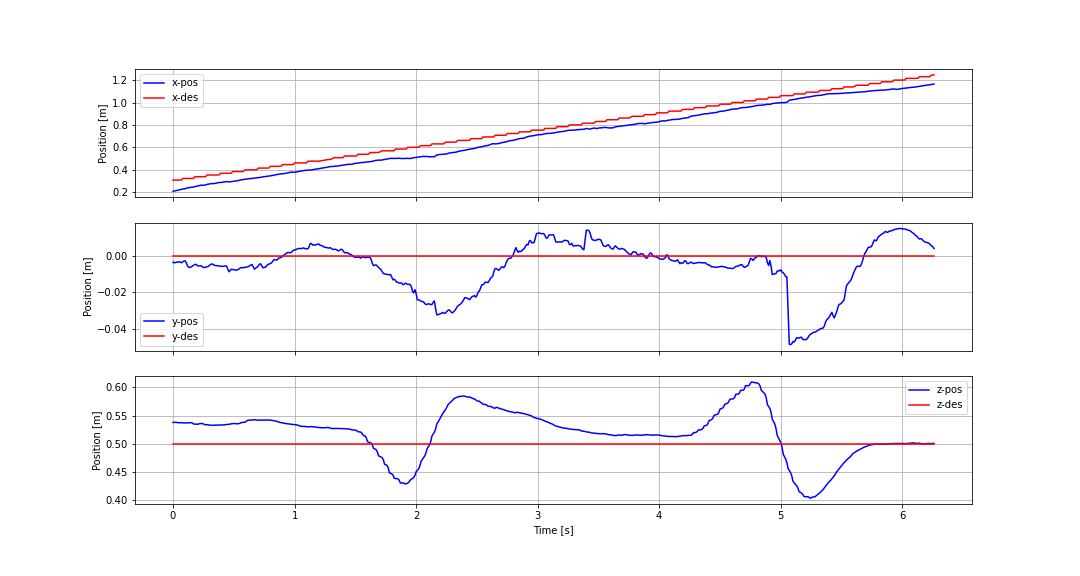
\includegraphics[width=1.0\linewidth]{Technical/m1.png}  
  \caption{Positional data versus time for straight line flight path over an object}
  \label{fig:m1}
\end{figure}

\subsubsection{Milestone 2: Map an Empty Grid}
This milestone was to have a successful flight in a lawnmower pattern over an empty grid and to visualize the topographical map of the empty grid. The topographic map of the empty grid is shown below in Figure \ref{fig:m2}.

\begin{figure}[H]
  \centering
  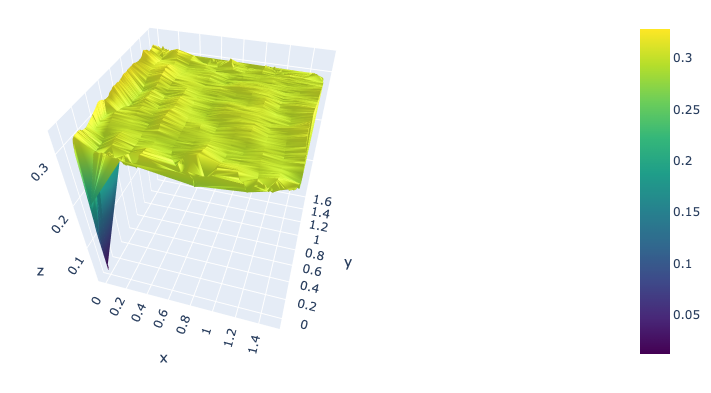
\includegraphics[width=0.8\linewidth]{Technical/m2.png}  
  \caption{Topographic map of empty grid}
  \label{fig:m2}
\end{figure}

\subsubsection{Milestone 3: Map an Object-filled Grid}
This milestone was to have a successful flight in a lawnmower pattern over an object-filled grid and to visualize the topographical map of the filled grid. This visualization is given below in Figure \ref{fig:m3}.

\begin{figure}[H]
  \centering
  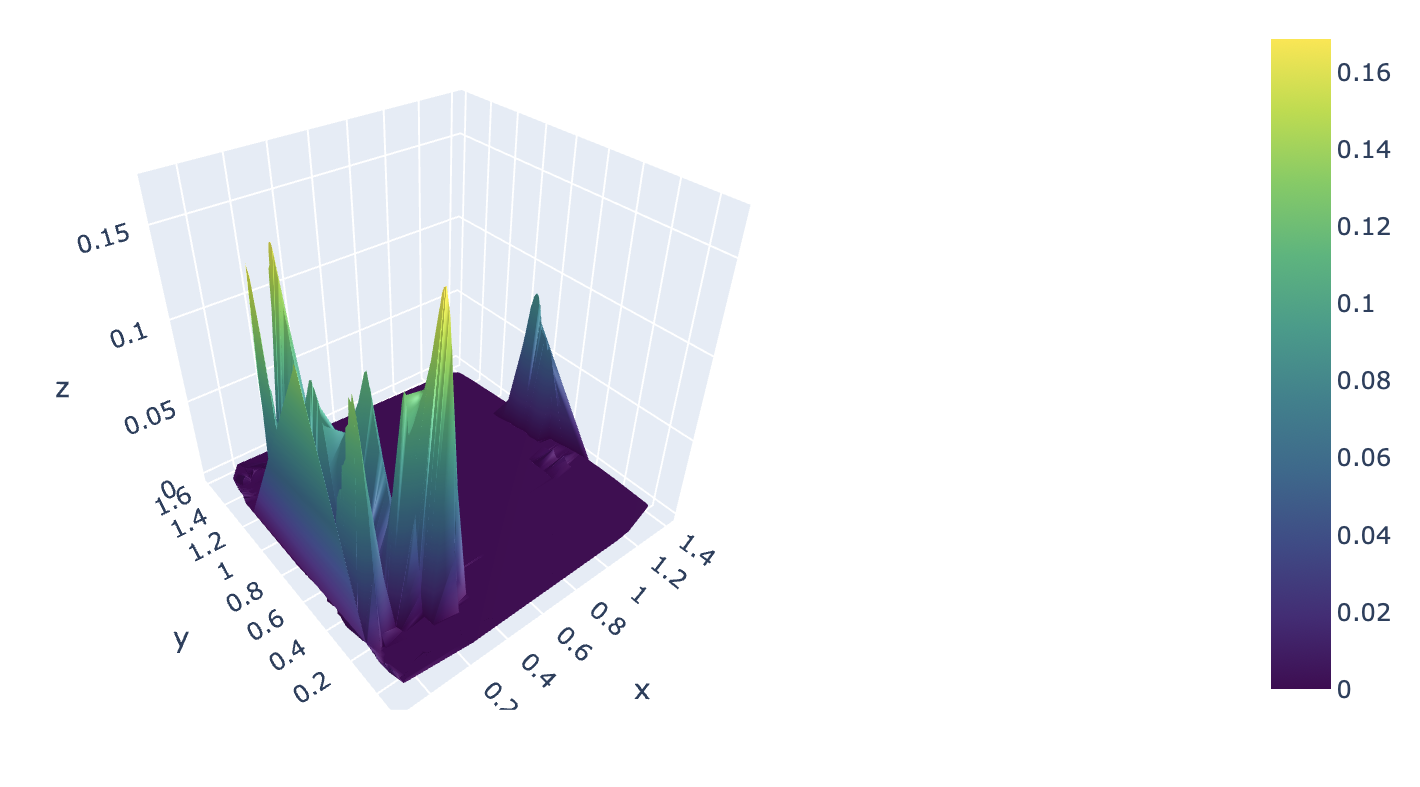
\includegraphics[width=0.8\linewidth]{Technical/m3.png}  
  \caption{Unprocessed topographic map of the object filled grid}
  \label{fig:m3}
\end{figure}

\subsubsection{Milestone 4: Visualization}
The final milestone was to produce the post-processed 3D topographical map of the object filled grid using Python. The produced visualizations were to be accurate replications of the real world object filled grid are shown and discussed in the results section.








\section{Implementation}
\label{Implementation}
The controller design that is derived in the following sections was not used due to its inability to have the drone follow the pattern shown on Fig \ref{fig:lawnmower}. The time constraint of the project made it impossible to change the controller design so that the drone could follow this pattern which is why the default controller and observer were used to collect all the data provided in Section \ref{R&D}.

\subsection{Equations of Motion}
The equations of motion for the drone are given as follows:
\begin{equation}
    \label{eqt 1}
    \dot{o}_{1}^{0} = R_{1}^{0}v_{0,1}^{1}
    \qquad\qquad
    \begin{bmatrix}
    \dot{\psi} \\ \dot{\theta} \\ \dot{\phi}
    \end{bmatrix} = N\omega_{0,1}^{1}
\end{equation}

\begin{equation}
    \label{eqt 2}
    f' = m\dot{v}'_{0,1} + \omega'_{0,1}\times (mv'_{0,1})
\end{equation}
\begin{equation}
    \label{eqt 3}
    \tau' = J'\dot{\omega}'_{0,1} + \omega'_{0,1}\times (J'\omega'_{0,1})
\end{equation}
where $R$ and $N$ are given as:
\begin{equation}
    R = \begin{bmatrix}
    \cos{\psi}\cos{\theta} & \sin{\phi}\sin{\theta}\cos{\psi}-\sin{\psi}\cos{\phi} & \sin{\phi}\sin{\psi}+\sin{\theta}\cos{\phi}\cos{\psi} \\
    \sin{\psi}\cos{\theta} & 
    \sin{\phi}\sin{\psi}\sin{\theta}+\cos{\phi}\cos{\psi} & -\sin{\phi}\cos{\psi}+\sin{\psi}\sin{\theta}\cos{\phi} \\ 
    -\sin{\theta} & \sin{\phi}\cos{\theta} & \cos{\phi}\cos{\theta}
    \end{bmatrix}
\end{equation}
\begin{equation}
    N = \begin{bmatrix}
    0 & \frac{\sin{\phi}}{\cos{\theta}} & \frac{\cos{\phi}}{\cos{\theta}} \\ 
    0 & \cos{\phi} & -\sin{\phi} \\
    1 & \sin{\phi}\tan{\theta} & \cos{\phi}\tan{\theta}
    \end{bmatrix}
\end{equation}
The drone has $12$ states, $4$ inputs and $5$ parameters as shown below:

\begin{equation}
  s = \begin{bmatrix} o_x \\ o_y \\ o_z \\ \psi \\ \theta \\ \phi \\ v_x \\ v_y \\ v_z \\ \omega_x \\ \omega_y \\ \omega_z \end{bmatrix}  
  \qquad\qquad
  i = \begin{bmatrix} \tau_x \\ \tau_y \\ \tau_z \\ f_z \end{bmatrix}  
  \qquad\qquad
  p = \begin{bmatrix} m \\ J_x \\ J_y \\ J_z \\ g \end{bmatrix}
\end{equation}

Rearranging equations \ref{eqt 1}-\ref{eqt 2}-\ref{eqt 3} in the form of $\dot{s} = f(s,i,p)$ results into the final form of the equations of motion:

\begin{equation}
   \begin{bmatrix} o_x \\ o_y \\ o_z \\ \psi \\ \theta \\ \phi \\ v_x \\ v_y \\ v_z \\ \omega_x \\ \omega_y \\ \omega_z \end{bmatrix}  = \begin{bmatrix}
   v_x\cos{\psi}\cos{\theta}+v_y(\sin{\phi}\sin{\theta}\cos{\psi}-\sin{\psi}\cos{\phi})+v_z(\sin{\phi}\sin{\psi}+\sin{\theta}\cos{\phi}\cos{\psi}) \\
   v_x\sin{\psi}\cos{\theta}+v_y(\sin{\phi}\sin{\psi}\sin{\theta}+\cos{\phi}\cos{\psi})+v_z(-\sin{\phi}\cos{\psi}+\sin{\psi}\sin{\theta}\cos{\phi}) \\ 
   -v_x\sin{\theta}+v_y\sin{\phi}\cos{\theta}+v_z\cos{\phi}\cos{\theta} \\
   \frac{\omega_{y}\sin{\phi}}{\cos{\theta}}+\frac{\omega_{z}\cos{\phi}}{\cos{\theta}} \\ 
   \omega_{y}\cos{\phi} -\omega_{z}\sin{\phi} \\
   \omega_x+\omega_{y}\sin{\phi}\tan{\theta}+\omega_{z}\cos{\phi}\tan{\theta} \\ 
   \vspace{1.5pt}
   \frac{gm\sin{\theta}+mv_{y}\omega_{z}-mv_{z}\omega_{y}}{m} \\
   \vspace{2.5pt}
   \frac{-gm\sin{\phi}\cos{\theta}-mv_{x}\omega_{z}+mv_{z}\omega_{x}}{m} \\
   \vspace{2.5pt}
   \frac{f_z-gm\cos{\phi}\cos{\theta}+mv_{x}\omega_{y}-mv_{y}\omega_{x}}{m} \\
   \vspace{2.5pt}
   \frac{J_{y}\omega_{y}\omega_{z}-J_{z}\omega_{y}\omega_{z}+\tau_x}{J_x} \\
   \vspace{2.5pt}
   \frac{-J_{x}\omega_{x}\omega_{z}+J_{z}\omega_{x}\omega_{z}+\tau_y}{J_y} \\ 
   \vspace{2.5pt}
   \frac{J_{x}\omega_{x}\omega_{y}-J_{y}\omega_{x}\omega_{y}+\tau_z}{J_z}
   \end{bmatrix} 
\end{equation}

The equations for the inputs can be written in terms of squared rotor speeds, $\sigma$s as follows:
\begin{equation}
    \begin{bmatrix} \tau_x \\ \tau_y \\ \tau_z \\ f_z \end{bmatrix}  =\begin{bmatrix}
    -lk_{F}\sigma_{1}^{2}-lk_{F}\sigma_{2}^{2}+lk_{F}\sigma_{3}^{2}+lk_{F}\sigma_{4}^{2} \\ 
     -lk_{F}\sigma_{1}^{2}+lk_{F}\sigma_{2}^{2}+lk_{F}\sigma_{3}^{2}-lk_{F}\sigma_{4}^{2} \\
      -k_{M}\sigma_{1}^{2}+k_{M}\sigma_{2}^{2}-k_{M}\sigma_{3}^{2}+k_{M}\sigma_{4}^{2} \\
      k_{F}\sigma_{1}^{2}+k_{F}\sigma_{2}^{2}+k_{F}\sigma_{3}^{2}+k_{F}\sigma_{4}^{2}
    \end{bmatrix}
\end{equation}

All the constant values like $m,J_x,J_y,J_z,g,l,k_F,k_M$ used in the above equations are given in Table \ref{Table 1}

\newpage
\begin{center}
\captionof{table}{\textbf{Constant Values used for the EOMs.}}

    \begin{tabular}{|c|c|}
        \rowcolor{lightgray} 
        \hline
        \textbf{Constant} & \textbf{Value} \\
        \hline
        m & 0.0313 kg \\
        \hline
        J_x & 1.80\times 10^{-5} kg-m^2 \\
        \hline
        J_y & 1.83\times 10^{-5} kg-m^2 \\
        \hline
        J_z & 3.17\times 10^{-5} kg-m^2 \\
        \hline
        g & 9.81 m/s^2 \\
        \hline
        l & 0.035 m \\
        \hline
        k_F & 2.04\times 10^{-6} \\
        \hline
        k_M & 7.51\times 10^{-9} \\
        \hline
\end{tabular}
\label{Table 1}
\end{center}

\subsection{State Space Model}
The state-space model was described from the EOMs as follows:

\begin{equation}
    \dot{s} = As+Bu
\end{equation}

where $x=s-s_{eq}$, $u=i-i_{eq}$. $A$ and $B$ were defined as:
\begin{equation}
    A = \frac{\partial f}{\partial s}\biggr\rvert_{(s_{e},i_{e},p_{e})} 
    \qquad\qquad
    B = \frac{\partial f}{\partial i}\biggr\rvert_{(s_{e},i_{e},p_{e})} 
\end{equation}

$s_{eq}$ and $i_{eq}$ were chosen as:

\begin{equation}
    s = \begin{bmatrix} 0 \\ 0 \\ 0 \\ 0 \\ 0 \\ 0 \\ 0 \\ 0 \\ 0 \\ 0 \\ 0 \\ 0 \end{bmatrix}  
  \qquad\qquad
  i = \begin{bmatrix} 0 \\ 0 \\ 0 \\ mg \end{bmatrix}
\end{equation}



\section{Controller Design}
\label{Controller}
For the controller, linear state feedback was applied:
\begin{equation}
    u = -K(s-s_{des})
\end{equation}

where $s_{des} = [o_{x,des}, o_{y,des}, o_{z,des}, 0,0,0,0,0,0,0,0,0]$ and $K$ was chosen by solving an infinite-horizon LQR problem.  

$Q$ and $R$ were chosen as follows:
\begin{equation}
    Q = \begin{bmatrix}
    30 \\ 27 \\ 520 \\ 200 \\ 25 \\ 25 \\ 1 \\ 1 \\ 0.17 \\ 1 \\ 1 \\ 100
    \end{bmatrix}
    \quad \quad
    R = \begin{bmatrix}
    6.297\times 10^6 \\ 6.297\times 10^6 \\ 5.692\times 10^8 \\ 7.714\times 10^3 
    \end{bmatrix}
\end{equation}

$K$ from LQR problem was:
\begin{equation*}
K = \left[ {\begin{array}{cccccccccccc}
    0 & -0.002 & 0 & 0 & 0 & 0.004 & 0 & -0.001 & 0 & 0.001 & 0 & 0\\
    0.002 & 0 & 0 & 0 & 0.004 & 0 & 0.001 & 0 & 0 & 0 & 0.001 & 0\\
    0 & 0 & 0 & 0 & 0 & 0 & 0 & 0 & 0 & 0 & 0 & 0\\
    0 & 0 & 0.260 & 0 & 0 & 0 & 0 & 0 & 0.128 & 0 & 0 & 0
    \end{array}}\right]

\end{equation*}





% \subsection{Milestone for Week of November 1}
% \label{MW1}
% The key milestone this week will be to understand and implement how to get the absolute and relative z-position of the drone. When attempting to create a topographical map of the grid that is being recorded, it is crucial to understand what data the drone is able to provide and how that data can translate into a topographical map. There are 2 ways that will be explored in understanding how to obtain the absolute and relative z-position of the drone. The first one is using a loco-positioning system, and the second one is using the z-position data of the drone. Understanding how to implement both methods will be the starting point after which the pros and cons of the different methods will be evaluated to determine the final method used in this project. Once a method is identified, it will be implemented in a flight test where the drone will be flown in a straight line over an object of known height. Then the z-data will be extracted to see if the drone was able to provide the x, y, and z position of the object. 

The first milestone for the week of November 1 was to identify the pros and cons of the 2 methods and choose the method best suited for this project. The pros and cons for both methods are given in Table \ref{Table 1}. The pros for the loco positioning system include the measurement of absolute z position and ability to map an object of unknown height. The cons for this same method are the unfamiliarity with the loco positioning system and the need for an additional deck, anchors, and tags which are quite expensive. Pros of the second method include the ease of implementation as well as no additional materials being needed. The downsides to this method are that measurement of objects of unknown height is not possible and that error in the data could be due to the controller as opposed to object detection. \\
Due to the time constraint of the project, the second method was chosen for the implementation.
\begin{center}
    \captionof{table}{\textbf{Pros and Cons for the 2 methods proposed}}
    {
    \medium
    
    \begin{tabular}{|c|c|c|}
        \rowcolor{lightgray}
        \hline
        {{\textbf{Method} & \textbf{Pros} & \textbf{Cons}}} \\
        \hline
        {\makecell{Loco Positioning \\ System} & \makecell{-Able to measure \\ absolute z position \\ -Map out the object \\ of unknown height}& \makecell{-Additional deck required \\ + anchors and tags \\ -Unknown deck, don't exactly know \\ how the loco positioning works}} \\
        \hline
        \makecell{z position data} & \makecell{-Easy to implement; \\don't need additional material \\ -Easy to implement because \\ the method is known}& \makecell{-Can't do unknown \\ object heights \\ -The error could be greater \\ because of the controller \\ which would result into inaccurate \\ topographical map}
        \\
        \hline
    \end{tabular}
    }
    \label{Table 1}
\end{center}

% \subsection{Milestone for Week of November 8}
% \label{MW2}
% The key milestone this week will be to have a successful flight in a lawnmower pattern over an empty grid and to visualize the topographical map of the empty grid. A visual representation of the pattern can be seen in Fig. \ref{lawnmower}.  The drone begins at the bottom left corner which will be defined as the origin (0,0). The end of the grid in coordinate system is (1.5,1.5). The dark blue lines depict the path of the drone moving forward to the end of the grid. The red dashed line depicts the drone returning back to origin from the end.\\
\indent A successful flight is defined by having the 6 states of interest be within the tolerances. Specifically the goal of the flight test is to ensure the error in the x,y,z position and the roll, pitch, and yaw angles are within tolerance. This allows the controller error to be minimized. The values that will be used for tolerance are:
{\renewcommand\arraystretch{1.0}
\noindent\begin{longtable*}{@{}l @{\quad \le \quad} l@{}}
$O_x$ & 0.075 m\\
$O_y$ & 0.075 m\\
$O_z$ & 0.075 m\\
$\psi$ & 0.05 \\
$\theta$ & 0.015\\
$\phi$ & 0.015\\
\end{longtable*}}
Once the RMSE of the 6 states are within the tolerance limits, a topographical map of the empty grid will be created. The analysis of the data collected by the drone as well as the plotting of the map will be done using python.



% \subsection{Milestone for Week of November 15}
% \label{MW3}
% The key milestone this week will be to have a successful flight in a lawnmower pattern over an object-filled grid and to visualize the topographical map of the filled grid. The drone will be flown over the grid and once again, the controller's error will be checked. The controller will be tweaked until the RMSE values, flying over an object-filled grid, are within tolerance in the x and y position, and $\psi$, $\theta$, and $\phi$.\\
\indent The flight of the drone will be modified such that when the drone senses it's height dropping (sensing the leading edge of the object) it will stop moving in the x and y direction, and will hover up to correct the relative z-position. Once it has reached it's "relative" height of 1m, the drone will be commanded to move forward until it senses that it is too high (sensing the trailing edge of the object). Then the drone will stop moving in the x and y position and will move back down to an absolute z-position of 1 m. This serves as further controller error mitigation enabling the distinguishing of z-range measurement changes due to topography. The x and y positions will be determined as well and the topographic data points will then be used to visualize a contour map of the filled grid. 



% \subsection{Milestone for Week of November 29}
% \label{MW4}
% The key milestone this week will be to use the final controller from the Week of November 15 to successfully produce a 3d topographical map of the object of the known height and 2d surface map. The produced visualizations should be accurate replications of the real world object filled grid. The same flight that as in the week of November 15 will be done. The x,y and z positions will be collected from this flight which then will be used to visualize a 3D topographical and 2D surface map of the filled grid using Python.

\section{Results and Discussion}
\label{R&D}
Once the experiment was complete, a number of different results were extracted. It was important to know how the drone flew over the grid in comparison to the desired flight path. Considering that the drone flew across the grid and flew back across the grid in a different configuration, the forward and backward flight path of the drone was plotted across the desired flight path. Fig. (\ref{fig:FFP}) and Fig. (\ref{fig:BFP}) show the forward and backward flight path of the drone as well as the coverage area over which objects were placed. The red region in the figures indicates the area of interest. This region is smaller than the drone flight path to mitigate errors arising from the turning switchback sections of the flight path.
\begin{figure}[H]
  \centering
  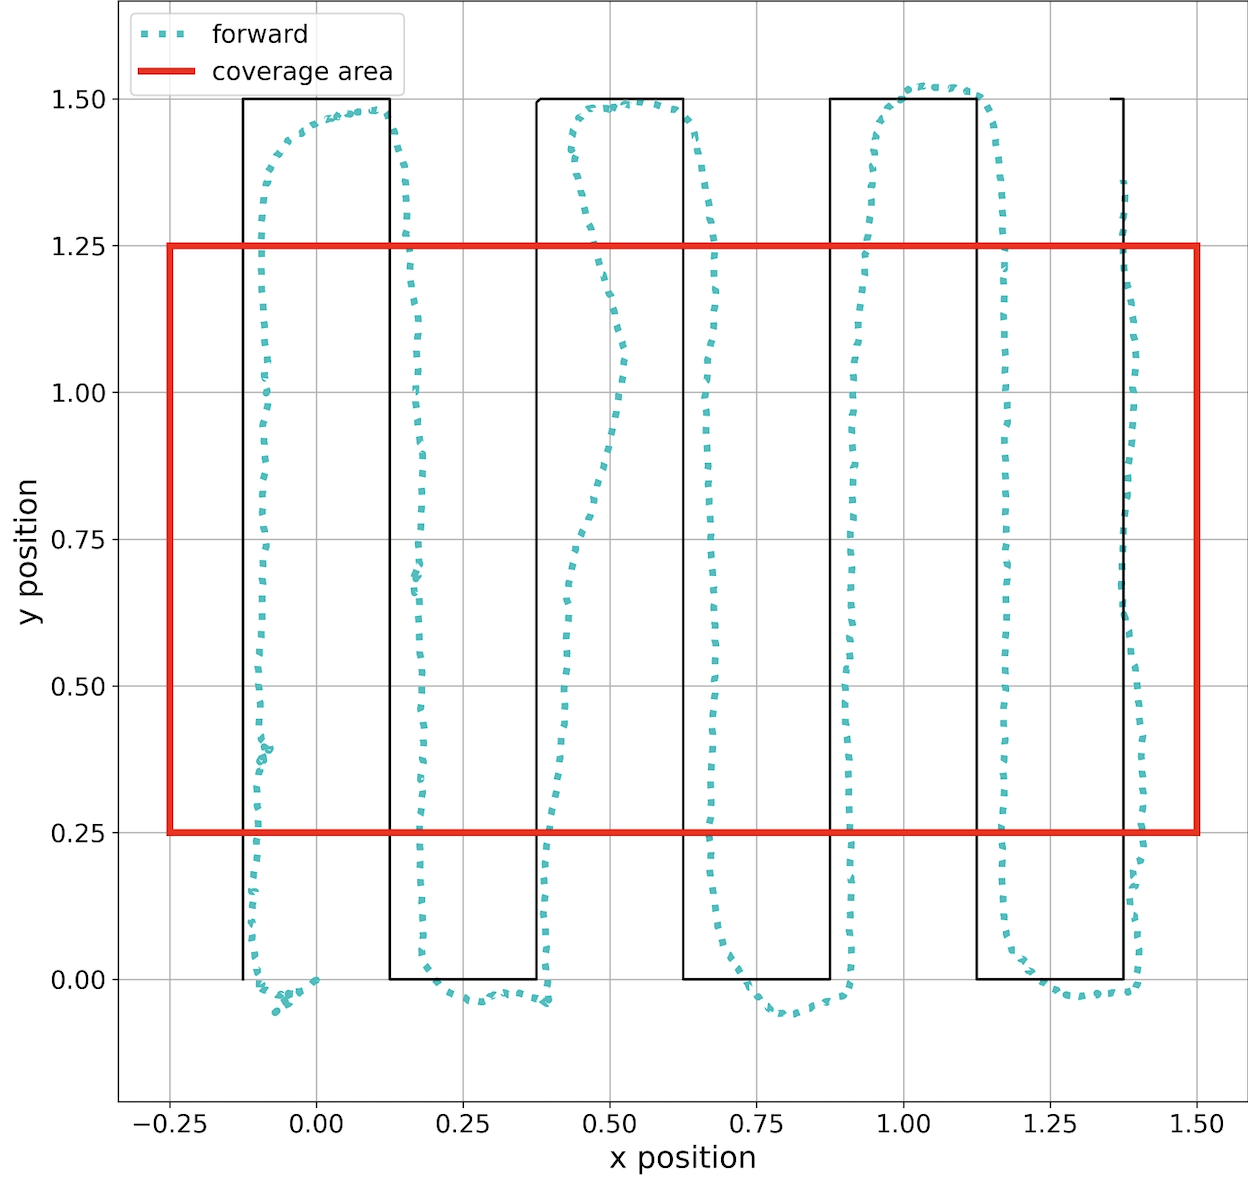
\includegraphics[width=0.7\linewidth, height=0.7\linewidth]{R&D/FFP.png}  
  \caption{Forward Flight Path}
  \label{fig:FFP}
\end{figure}

From Fig. (\ref{fig:FFP}) it is clear that the drone flew pretty close to the desired flight path going forward (left to right) across the grid. The red lined box represents the area in which objects were placed to provide the drone more time to stabilize once it cleared the object filled regions. Objects weren't placed all over the area of coverage, just in certain regions, to provide a more realistic grid to map out. We see at points in time where it deviates from the desired flight path, and the reason for this was that an object was placed there, and whenever the drone sensed the edge of an object, it increased the z-position that it was flying at, and that sudden increases caused it to lose control and stability a little bit, resulting in the drone not flying on the desired flight path. Whenever the drone was flying over the center of an object, it is seen that the drone did not deviate as much from the desired flight path. Between 0.375 m and 0.5 m in the x position, the drone is seen to deviate the most, and this was a result of the edge of an object being located there, which was a challenge faced using just the flow deck. Complex configurations of objects could not be flown over without deviation, which is where the loco-positioning system would have provided more accurate results. Regardless of these deviations, as shown in Fig. (\ref{fig:PvsT}), the actual flight path of the drone was not far from the desired flight path of the drone in terms of its x and y position. 

\begin{figure}[H]
  \centering
  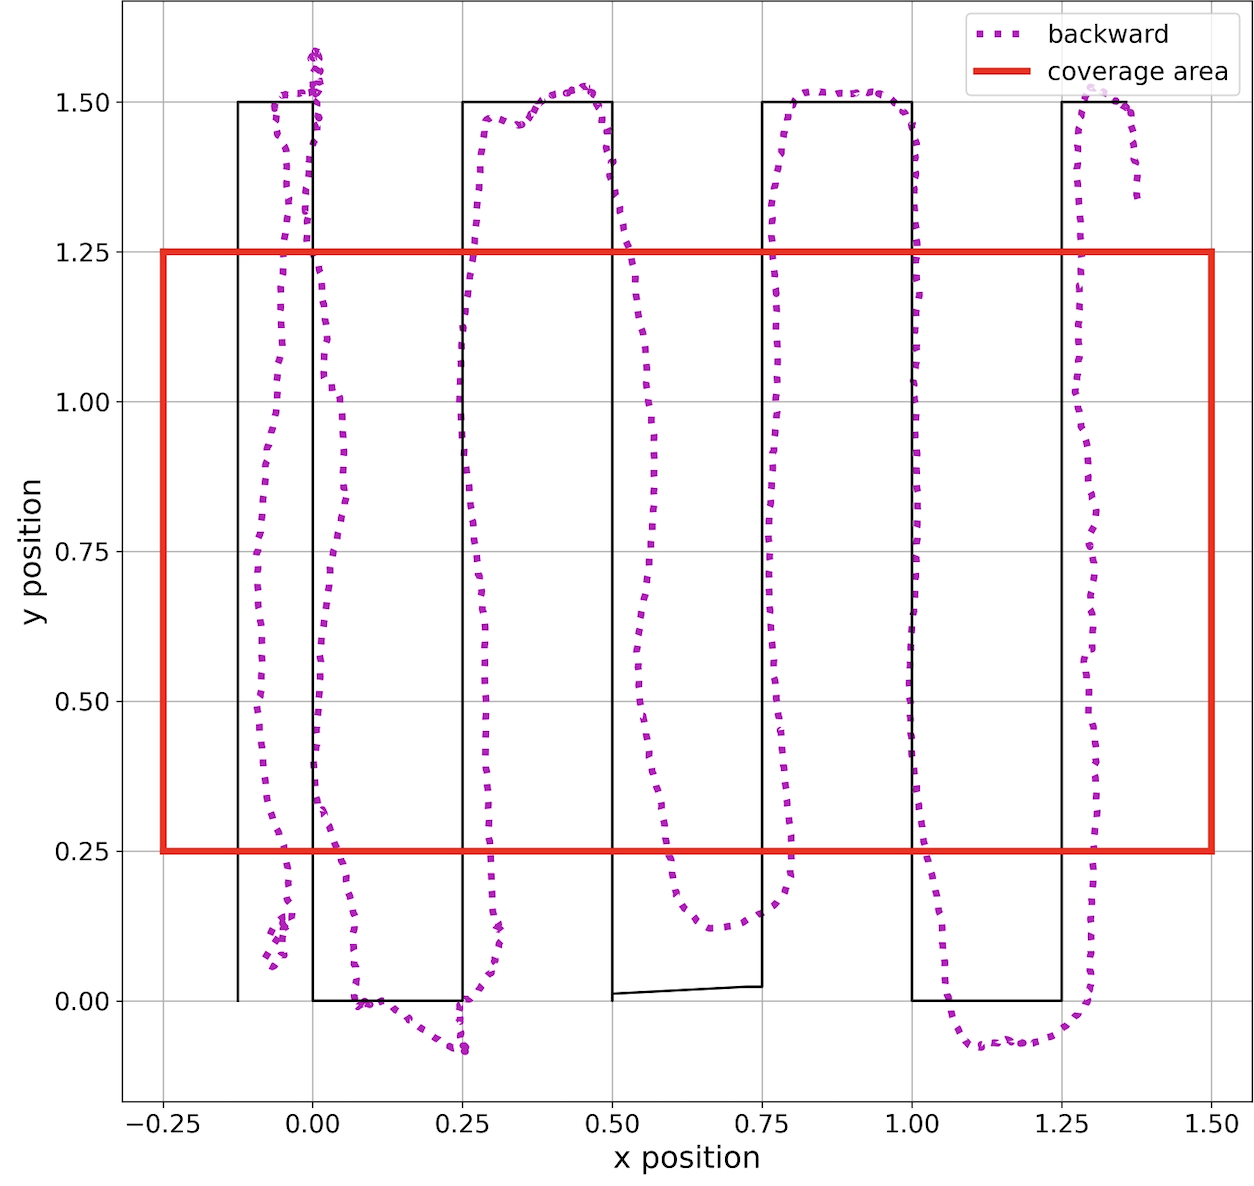
\includegraphics[width=0.7\linewidth, height=0.7\linewidth]{R&D/BFP.png}  
  \caption{Backward Flight Path}
  \label{fig:BFP}
\end{figure}

Fig. (\ref{fig:BFP}) shows the backward flight path (right to left) of the drone, to go from a location of (1.5 m, 1.5 m) in the (x,y) position back to origin, located at (0,0). The initial movement to turn back around to fly back to origin was a sharper turn than normal ones, with a distance of only 0.125 m. The drone is seen to follow a the desired flight path pretty accurately for the first couple turns, but at around a similar position as seen in Fig. (\ref{fig:FFP}), the drone is seen to deviate from the desired flight path as it hits the edge of an object. Similarly, near the end of the flight of the drone, we see the drone going a little haywire, and losing control as it hits the edge of another object - a result of a modified flight path. During forward motion, the drone flew over the center of the object, which caused it to remain stable, but on the way back, it sensed the edges, which is something that the group wanted to test out; the reaction of the drone flying over the edges of the object. This resulted in the drone taking a lot longer to stabilize considering the drone didn't sense it with the entire camera because of the camera's FOV, and that resulted in the drone moving in the North-west direction in the z-axis rather than just north. Therefore, from both the forward and backward flight path graphs, it is evident that the drone worked best when its camera's FOV was only sensing a completely flat surface rather than different altitude surfaces. To ensure that the path of the drone in both the x and y direction was identical or similar to the provided inputs, a plot of the x and y position of the drone was plotted against its desired x and y position.

\begin{figure}[H]
  \centering
  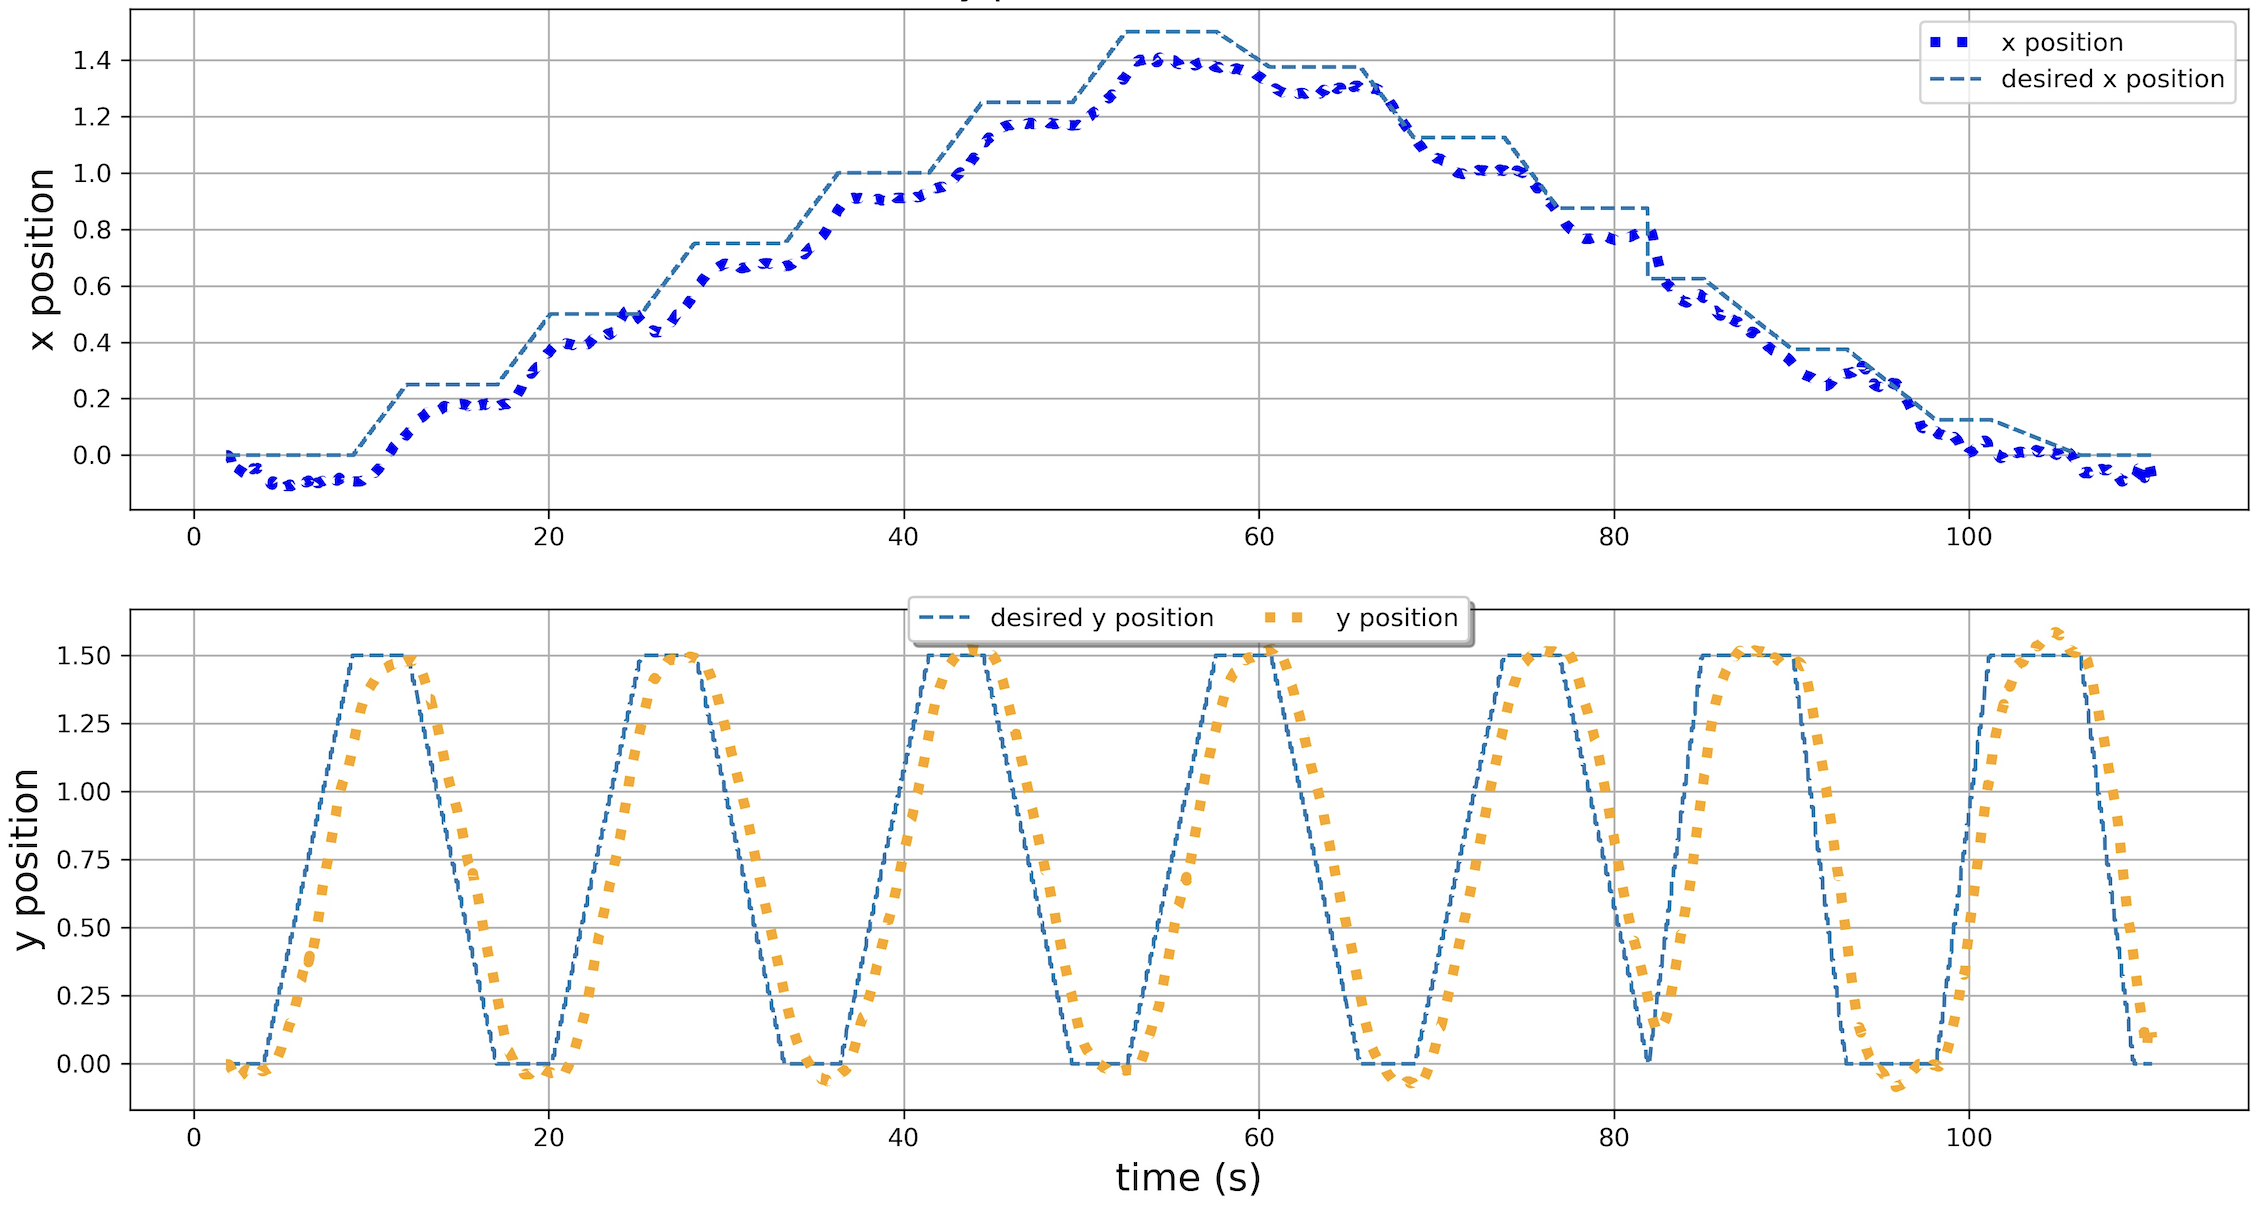
\includegraphics[width=0.8\linewidth, height=0.6\linewidth]{R&D/PvsT.png}  
  \caption{X and Y Position vs. Time}
  \label{fig:PvsT}
\end{figure}

Fig. (\ref{fig:PvsT}) shows the x and y position of the drone and the desired x and y position of the drove against time. The total flight time for the drone to complete the entire forward and backward flight path was about 112 seconds. Our initial tests completed the entire flight in a much shorter period of time, but the trade off was that the drone was not as stable, and was not tracking the desired positions as accurately as our final test. As the graph shows, at a slower speed, the drone was able to fly over the object filled grid more accurately with a slight offset in the x position (in a negative manner), and a slight offset in the y position in terms of at what time it went over the desired y positions. From the x-position graph, we can see that at the start, the drone sweep-ed a little bit when taking off, causing it to go into the negatives of the x-position, which is why throughout the flight test, it was about 0.05 m off the desired x-position. From the y-position graph, we can see that at the start, there was also a delay in terms off the drone taking off, resulting in it being offset to the desired y position by about 1.5 seconds. There are some larger deviations seen in the graph from the desired position, where the graph is not following the trend of the desired x and y position, and these occurred when the drone flew over an edge of an object, and this was an expected result for the team. When implementing the project using just the flow deck, there was a trade-off between using the loco-positioning system and just the flow deck, and that was based off of the complexity of objects that the drone would be able to successfully fly over to create a topographical map. Overall, the graphs show that the drone was able to fly across the grid close to the desired positions provided to the drone. The RMSE values of the drone flight over the empty grid and the object filled grid are given in the tables below.

\begin{center}
\captionof{table}{\textbf{RMSE Values of Drone Flight with Targets for Empty Grid}}

    \begin{tabular}{|c|c|c|}
        \rowcolor{lightgray} 
        \hline
        \textbf{State} & \textbf{Experimental RMSE} & \textbf{Target RMSE} \\
        \hline
        o_x & 0.0134 & 0.075 \\
        \hline
        o_y & 0.190 &  0.075  \\
        \hline
        o_z & 0.016 &  0.075  \\
        \hline
        \psi & 0.011 &  0.050  \\
        \hline
        \theta & 0.014 &  0.015 \\
        \hline
        \phi & 0.014 &  0.015 \\
        \hline
\end{tabular}
\end{center}

\begin{center}
\captionof{table}{\textbf{RMSE Values of Drone Flight with Targets for Object Filled Grid}}

    \begin{tabular}{|c|c|c|}
        \rowcolor{lightgray} 
        \hline
        \textbf{State} & \textbf{Experimental RMSE} & \textbf{Target RMSE} \\
        \hline
        o_x & 0.095 & 0.075 \\
        \hline
        o_y & 0.229 &  0.075 \\
        \hline
        o_z & 0.479 &  0.075 \\
        \hline
        \psi & 0.011 &  0.050 \\
        \hline
        \theta & 0.014 &  0.015 \\
        \hline
        \phi & 0.014 &  0.015 \\
        \hline
\end{tabular}
\end{center}

\begin{figure}[H]
\centering
\begin{subfigure}{0.9\textwidth}
  \centering
  % include First image
  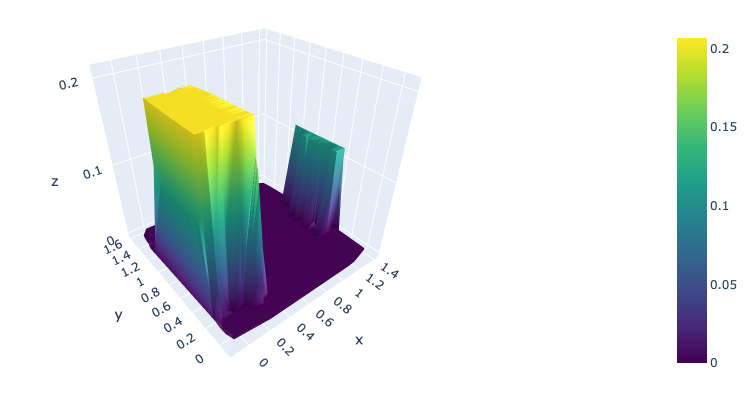
\includegraphics[width=0.85\linewidth]{R&D/3Dplot1.png}
  \caption{View 1}
  \label{fig:F3DP}
\end{subfigure}
\begin{subfigure}{0.9\textwidth}
  \centering
  % include Second image
  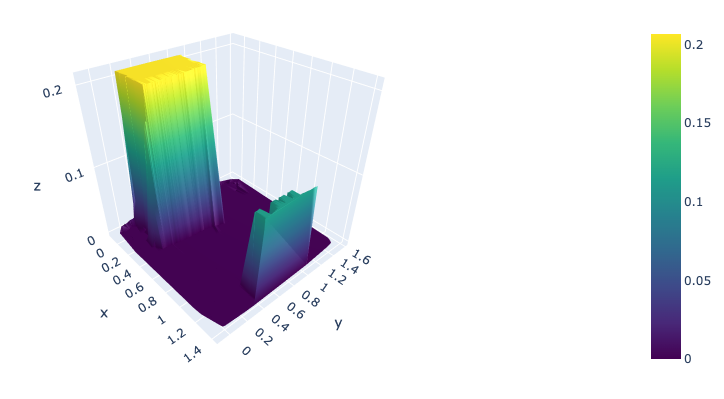
\includegraphics[width=0.85\linewidth]{R&D/3Dplot2.png}
  \caption{View 2}
  \label{fig:B3DP}
\end{subfigure}
\caption{Post-Processed Topographical Visualization of the location the Drone Flew Over}
\label{fig:3DP}
\end{figure}

Fig. (\ref{fig:3DP}) shows a successful visualization of the object filled grid. Both the forward and backward flight were used to create a post-processed topographical visualization of the grid. Objects were placed as shown in Fig. (\ref{fig:OFG}), and from Fig. (\ref{fig:F3DP}) and Fig. (\ref{fig:B3DP}) the approximate (x,y,z) positions of the objects can be seen. 

Post processing was done by first getting the (x,y) locations of the first and last peaks in the flight path for each object as shown in the figure \ref{fig:r1}. From these locations, and because it was known that the objects were rectangular, the area of the objects could be determined. It is necessary to note that due to not using the loco-positioning deck, the unobservability of the x and y positions cause significant drift in the x and y directions. The actual and experimentally determined x and y dimensions of the objects are given in the table below. With more testing correction factors could be developed to mitigate the error in these measurements if the loco-positioning deck is not used. From the current testing done a correction factor of $75\%-80\%$ could be employed to get the proper (x,y) dimensions of the objects.

\begin{center}
\captionof{table}{\textbf{Brown Box Dimensions}}

    \begin{tabular}{|c|c|c|}
        \rowcolor{lightgray} 
        \hline
        \textbf{Actual [cm]} & \textbf{Experimental [cm]} & \textbf{Percent Error [\%]} \\
        \hline
        x = 16.5 & x = 29 & 75.76 \\
        \hline
        y = 38 & y = 68 &  78.95 \\
        \hline
\end{tabular}
\end{center}

\begin{center}
\captionof{table}{\textbf{Black Box Dimensions}}

    \begin{tabular}{|c|c|c|}
        \rowcolor{lightgray} 
        \hline
        \textbf{Actual [cm]} & \textbf{Experimental [cm]} & \textbf{Percent Error [\%]} \\
        \hline
        x = 10 & x = 18 & 80.00 \\
        \hline
        y = 24.5 & y = 44 & 79.59\\
        \hline
\end{tabular}
\end{center}

\begin{figure}[H]
  \centering
  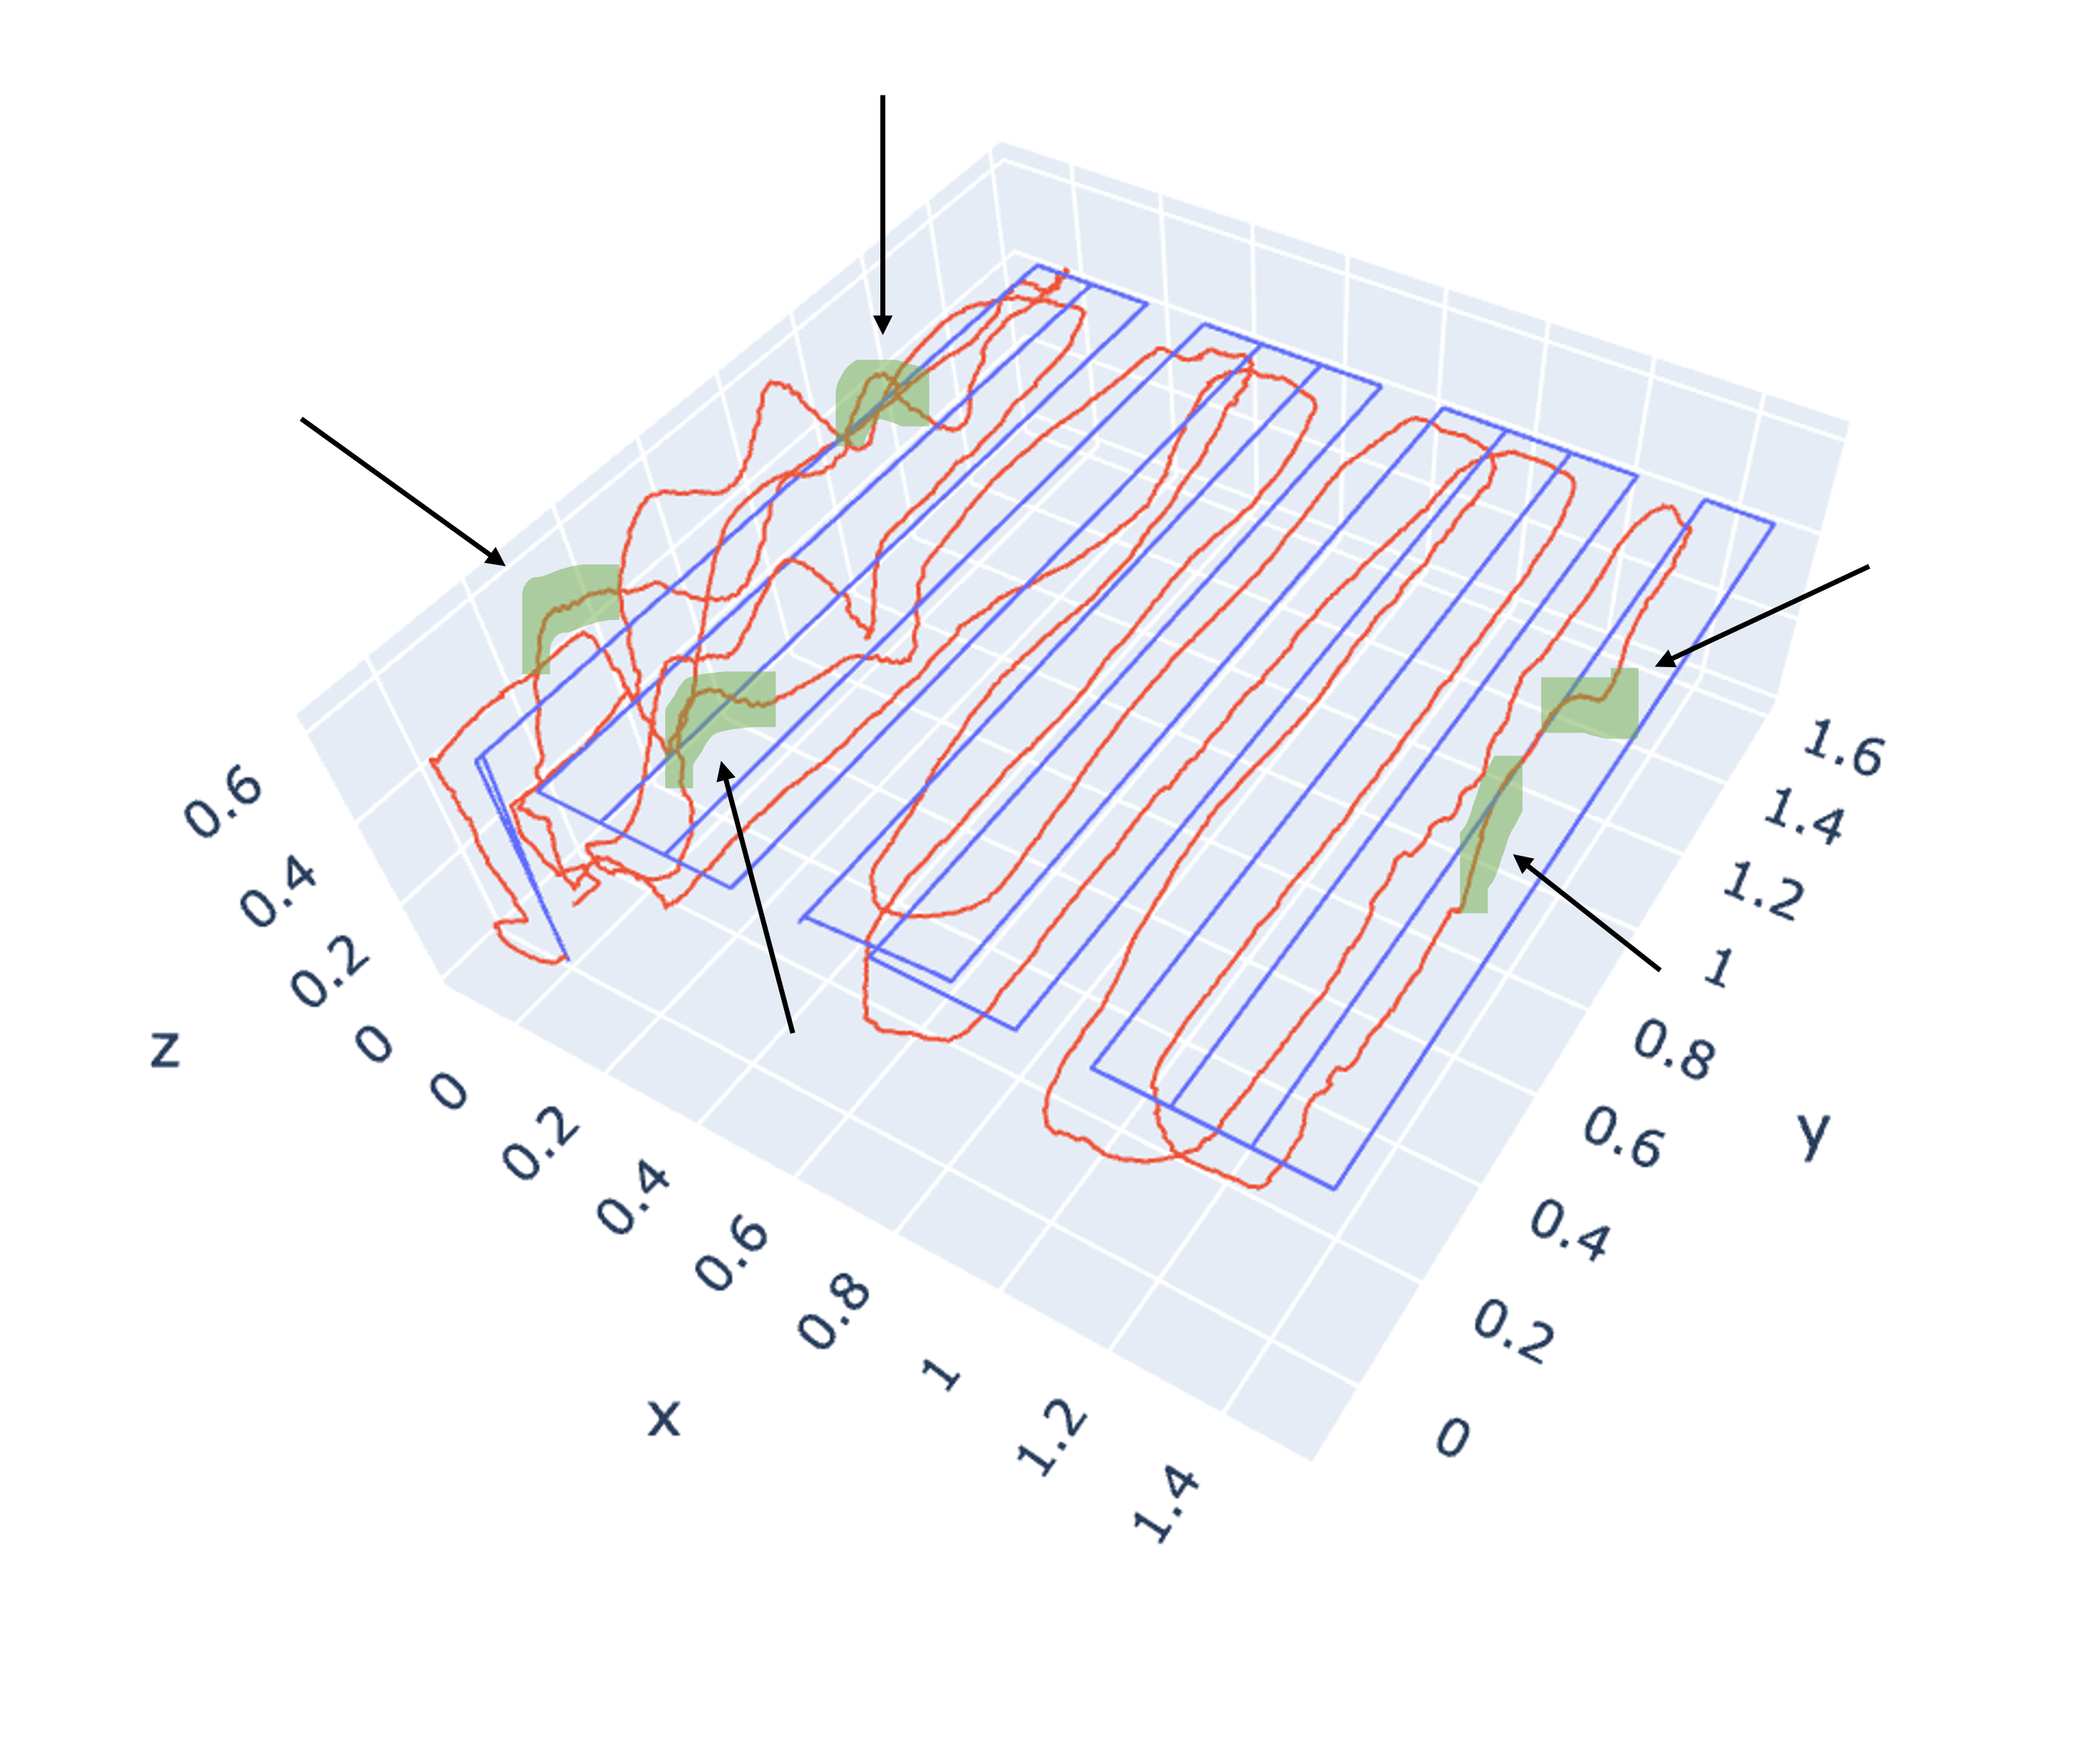
\includegraphics[width=0.8\linewidth]{R&D/r1.png}  
  \caption{Peaks in 3D Flight Path for (x,y) Approximate Position Extraction}
  \label{fig:r1}
\end{figure}

The z-direction measurements are much more accurate due to the observability of the state. For conciseness the process for determining the height of the brown box is detailed below; the procedure for the black box is identical. The z-position was extracted by subtracting the peak heights, indicated by the orange arrows, from the subsequent hover heights, indicated by the yellow highlight in the figure \ref{fig:r2}. The hover heights were average over a slice of time as the drone did not hover at exactly 0.45 m. After averaging all of the values from each peak and hover pair, the final height of the brown box was determined to be $0.1732$ meters. When compared with the actual object height of $0.2050$ meters, the margin of error was $15.51\%$. Following a similar procedure for the black box, the experimentally determined height was $0.0848$ meters, the actual height was $0.12$ meters, and the margin of error was $5.67\%$. A correction factor was applied by averaging the difference between the experimental and actual values for both objects. After the correction factor, which was $0.0335$, was applied the new z-positions were $0.2067$ and $0.1183$ with margins of error $0.83 \%$ and $1.42 \%$. All of this data has been tabulated below.

\begin{center}
\captionof{table}{\textbf{Object Heights}}

    \begin{tabular}{|c|c|c|c|}
        \rowcolor{lightgray} 
        \hline
        \textbf{Object} & \textbf{Actual [cm]} & \textbf{Experimental [cm]} & \textbf{Percent Error [\%]} \\
        \hline
        Brown Box & z = 17.32 & z = 20.50 & 15.51\%\\
        \hline
        Black Box & z = 8.48 & z= 12.00 &5.67\% \\
        \hline
\end{tabular}
\end{center}

\begin{center}
\captionof{table}{\textbf{Object Heights After Correction}}

    \begin{tabular}{|c|c|c|c|}
        \rowcolor{lightgray} 
        \hline
        \textbf{Object} & \textbf{Actual [cm]} & \textbf{Experimental [cm]} & \textbf{Percent Error [\%]} \\
        \hline
        Brown Box & z = 20.67 & z = 20.50 & 0.83\%\\
        \hline
        Black Box & z = 11.83 & z= 12.00 & 1.42\% \\
        \hline
\end{tabular}
\end{center}

\begin{figure}[H]
  \centering
  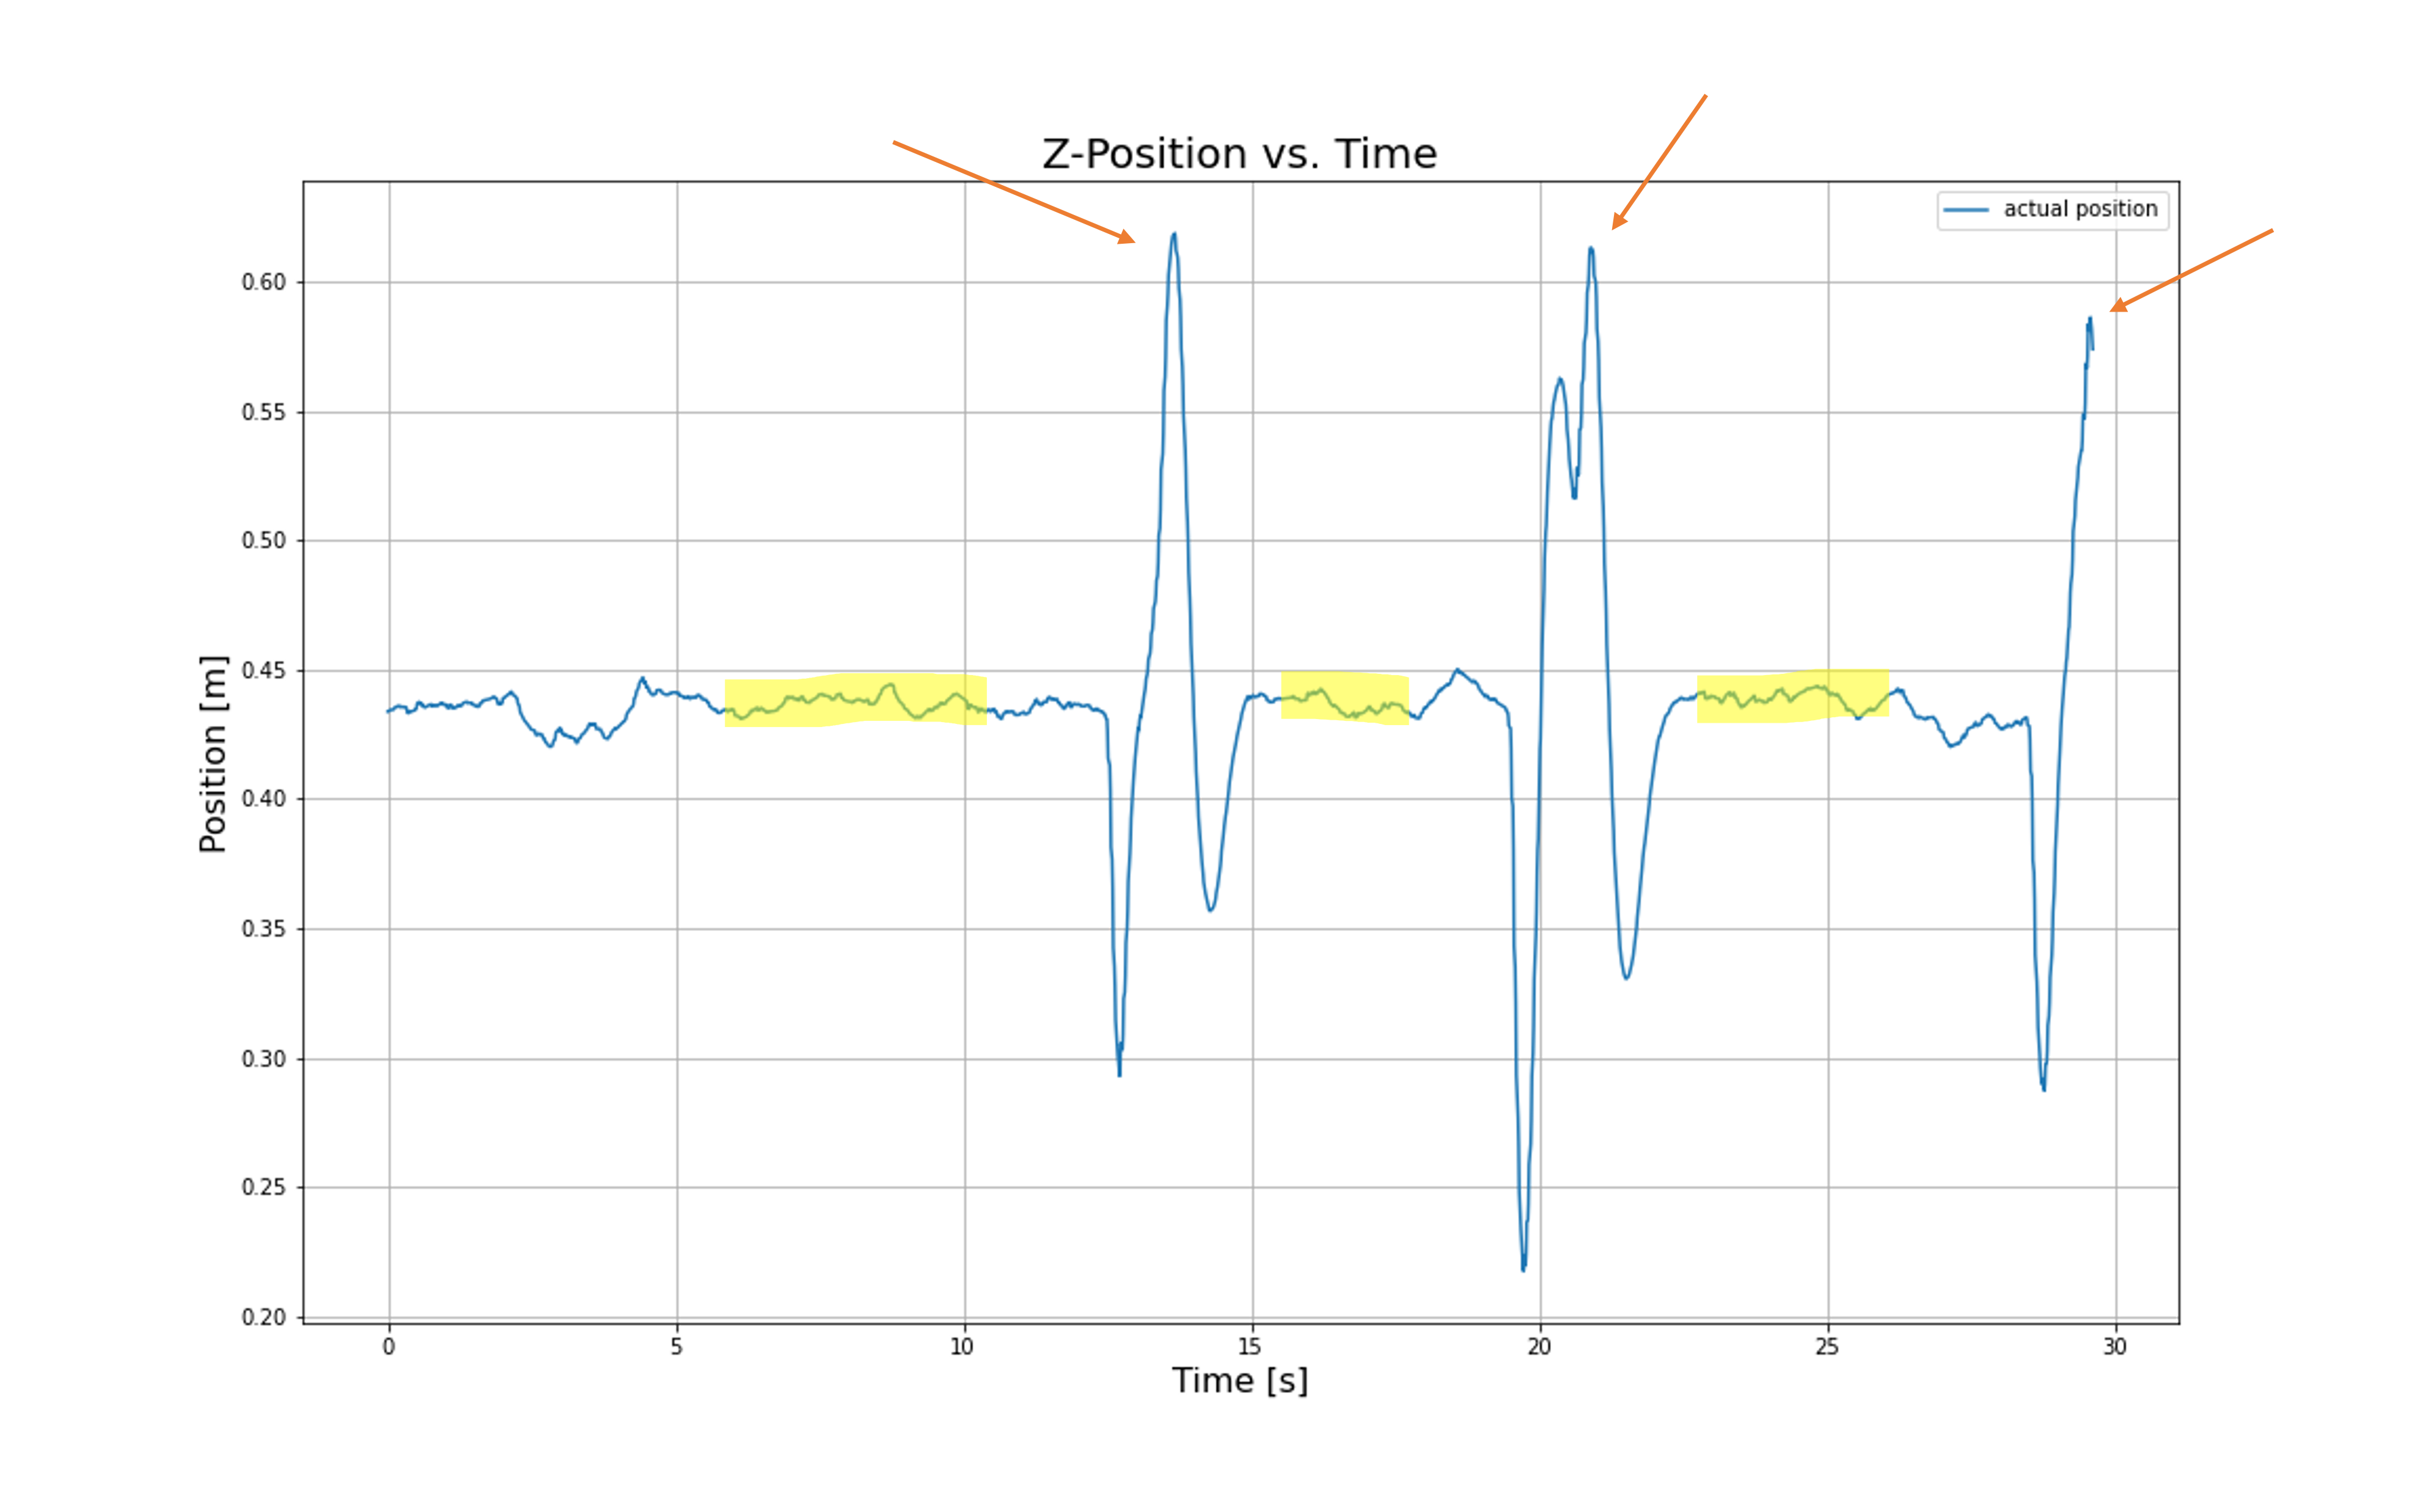
\includegraphics[width=1.0\linewidth]{R&D/r2.png}  
  \caption{Peaks in Z-Position vs. Time for Z-Position Extraction}
  \label{fig:r2}
\end{figure}

Once all of the positional information was determined the plot was smoothed out by subtracted the flight altitude from the z-positional data. This was done to make the floor of the test section coincide with the "floor" in the map. Then from the range of (x,y) values the z-positional data was modified to be that of the corrected object heights respectively. This resulted in the final plots shown above. Overall, the graphs that were visualized were accurate and provided a pretty good representation of the grid that the drone was flying over. The area the objects cover is larger than in actuality, however the true object locations are encompassed by this area. In addition this can be corrected by using a correction factor or loco-positioning deck as discussed. The group was able to show that the drones basic flow deck could be implemented when mapping out various different surfaces to provide a good approximation of what the surface in question would look like.


\section{Conclusions}
\label{Conclusions}
The final results can help draw several conclusions. Overall, the crazyflie drone's positioning capabilities using the flow deck were sufficient to create a three-dimensional topographical map of the grid that the micro-quadcopter flew over. The basic flight pattern used was of a switch back pattern, as shown in Fig. (\ref{fig:lawnmower}). There were many challenges that had to be overcome during the project. Firstly, the custom controller and observer caused the drone to swerve away from the desired flight path, due to which the stock controller and observer had to be used. Secondly, at higher velocities, the drone went haywire attempting to fly over an object filled grid, and for that reason, a slower forward-moving velocity had to be used. Thirdly, to ensure that there was full coverage of the 1.5 m x 1.5 m grid, the flight path had to be changed so that the drone would sweep around the edges of the grid to provide it more time to re-stabilize such that lower RMSE values were obtained. Lastly, the flight of the drone moving forward induced a sweep, where there was positive pitch induced on the drone, which resulted in the drone registering the (x,y) position with a delay, which was accounted for in python when using the geospatial data to visualize the topographical map.\\
\indent As seen from the experimental results, the drone was able to fly according to the desired flight path, with only some deviation. The drone's x position was slightly offset in the negative direction from the desired x-position, and the drone's y position was slightly offset to the right from the desired y-position. Overall, the drone's RMSE values in the x and y position were within tolerance. The topographical map produced using python showed the object-filled grid's surface visualization accurately, following the desired flight path that was provided to the drone. However, the dimensions of the box are not accurate, even though the locations and the fact that there is an object there is accurate. The drone was able to record the x and y position of these objects relatively well for lack of the states being observable, and the surface visualization represented the object-filled grid to a high degree of accuracy.\\
\indent However, this project can be improved upon in various ways if tested again in the future. One such improvement is detailed below. The flight of the drone could be modified such that when the drone senses it’s height dropping (sensing the leading edge of the object) it will stop moving in the x and y direction, and will hover up to correct the relative z-position. Once it has reached it’s "relative" height of 1m, the drone will be commanded to move forward until it senses that it is too high (sensing the trailing edge of the object). Then the drone will stop moving in the x and y position and will move back down to an absolute z-position of 1 m. This serves as further controller error mitigation enabling the distinguishing of z-range measurement changes due to topography. The x and y positions will be determined as well and the topographic data points will then be used to visualize a contour map of the filled grid.

Other improvements include implementing a custom controller and observer that was stable and observable would allow for a more stable flight with the drone being able to follow the desired flight path in a more accurate manner. Secondly, implementing a Loco-positioning system would increase the accuracy of results that are obtained, and it would allow mapping of more complex objects. However, the loco-positioning system also requires an extra deck, as well as anchors and tags, which increases the cost of the experiment, as well as the complexity of the project and it's implementation. Furthermore, if the project was able to be implemented on a surface that was not fixed, it would improve the application of the project - being able to track moving objects would allow the visualization of moving animals in forests or the movement of rocks/trees due to weather conditions, improving the extent of visualization provided. Lastly, being able to improve the stability of the drone would improve the application of this project through varying initial conditions not affecting the flight of the drone, and external factors not playing a role in the flight path of the drone. Overall, the project was a great success, and the results we got were accurate and what we expected, despite the challenges down the road.




\section*{Acknowledgments}
\label{Acknowledgements}
The group thanks 'Tim Bretl' for providing the possible solutions to obtaining the absolute and relative z-position of the drone, as well as debugging issues regarding the drone not collecting data during flight tests. \\
\indent Parthiv Kukadia and Pallavi Ravada thank 'Travis Zook' for helping brainstorm potential challenges that could be faced implementing a loco-positioning system and understanding how to extract the absolute and relative z-position using the flow deck.\\
\indent Ani Pirosmanishvili and Salam Mulhem thank 'Max Kolarich'$^*$ for helping us conduct the flight tests and extracting position and orientation of the drone from the stock controller. \\
\indent The group thanks Dan Block for providing the crazy-flie drone, the flow deck, as well as the lab space for testing.

\section*{References}
\label{Referenes}
[1] Perroud, D., “Surveying with a drone - what are the benefits and how to start?,” Wingtra Available:

\hspace{4.5mm} https://wingtra.com/drone-mapping-applications/surveying-gis/. 

[2] I. Gilbert, T. Vardhan, and K. Xu, “AE483 Final Project Thermal Mapping,” AE483 Final Project Report, 

\hspace{4.5mm} University of Illinois at Urbana-Champaign, Fall 2019.

[3] J. Morich, A. Hewson, and K. Pieper, “AE483 Final Project Sound Mapping with Quadrotor,” AE483 Final 

\hspace{4.5mm} Project Report, University of Illinois at Urbana-Champaign, Fall 2014.

[4] Arnaud, “Z-ranger and flow decks with improved range,” Bitcraze Available: https://www.bitcraze.io/2018/12/z-

\hspace{4.5mm} ranger-and-flow-decks-with-improved-range/. 

[5] K. Lohan, T. Jansen, and P. Rostkowski, “AE483 Final Project Covering and Mapping an Area,” AE483 Final 

\hspace{4.5mm} Project Report, University of Illinois at Urbana-Champaign, Fall 2014.

[6] A. Hong and C. Nunes, “AE483: Final Project Report,” AE483 Final Project Report, University of Illinois at 

\hspace{4.5mm} Urbana-Champaign, Fall 2014.

[7] A. Cichon, M. Danendra and A.E Strauch, "Search-and Rescue Object Detection", AE483 Final Project Report, 

\hspace{4.5mm} University of Illinois at Urbana-Champaign, Fall 2019.




\end{document}
